\documentclass[12pt,letterpaper]{article}

\usepackage{fontspec}
\setmainfont{Times New Roman}
\usepackage{polyglossia}
\setdefaultlanguage{spanish}

\usepackage[margin=2.5cm]{geometry}
\usepackage{graphicx}
\usepackage{booktabs}
\usepackage{array}
\usepackage{caption}
\usepackage{float}
\usepackage[table]{xcolor}
\usepackage{fancyhdr}
\usepackage[hidelinks]{hyperref}
\usepackage{enumitem}
\usepackage{tabularx}

\linespread{1.15}
\setlength{\parskip}{0.55em}
\setlength{\parindent}{0pt}
\captionsetup{font=small,labelfont=bf,skip=4pt}

\definecolor{ink}{HTML}{1B2733}
\definecolor{muted}{HTML}{55606C}
\definecolor{azul}{HTML}{1F4E79}
\definecolor{azulcl}{HTML}{9DBBD9}
\definecolor{gris}{HTML}{B9C0C8}
\definecolor{naranja}{HTML}{D9661F}
\definecolor{naranjatx}{HTML}{A84A12}
\definecolor{panel}{HTML}{F2F5F8}
\newcommand{\muestra}[1]{\textcolor{#1}{\rule{1.6em}{0.9em}}}

\pagestyle{fancy}
\fancyhf{}
\fancyhead[L]{\small CC3084 --- Laboratorio 9: Visualización estática}
\fancyhead[R]{\small\thepage}
\renewcommand{\headrulewidth}{0.4pt}

\begin{document}

%======================= PORTADA =======================
\begin{titlepage}
\centering
\vspace*{1.2cm}
{\large Universidad del Valle de Guatemala}\\[0.2em]
{\large Facultad de Ingeniería}\\[0.2em]
{\large Departamento de Ciencias de la Computación}\\[0.2em]
{\large CC3084 --- Data Science --- Semestre II, 2026}

\vspace{3cm}
\rule{\textwidth}{1.2pt}
\vspace{0.7cm}

{\Huge\bfseries Laboratorio 9}\\[0.6em]
{\LARGE Visualización estática}\\[0.9em]
{\large Documento de explicación de las decisiones de diseño}\\[0.3em]
{\large Infografía: \textit{El turismo de Guatemala ya superó la pandemia}}

\vspace{0.7cm}
\rule{\textwidth}{1.2pt}

\vspace{2.4cm}
{\large\bfseries Integrantes}\\[0.8em]
{\large Rodrigo Ajmac --- 22279}\\[0.3em]
{\large Andrés Mazariegos --- 21749}\\[0.3em]
{\large June Herrera --- 231038}

\vfill
{\large Guatemala, 15 de octubre de 2026}
\end{titlepage}

\tableofcontents
\newpage

%======================= 1 =======================
\section{Propósito, audiencia y pregunta guía}

La infografía sintetiza en una sola página los resultados del Laboratorio~1 (análisis
exploratorio, descomposición, pruebas de estacionariedad, diez modelos de pronóstico por serie y
sus métricas de error) para un \textbf{directivo del INGUAT que no es estadístico}. Esa audiencia
define todas las decisiones posteriores: el lector dispone de poco tiempo, necesita conclusiones
antes que procedimientos y debe poder actuar con lo que lee.

La pieza responde a la pregunta del enunciado: \textit{¿qué nos enseñan 17 años de datos
migratorios sobre el turismo en Guatemala y qué debemos anticipar hacia el futuro?} La respuesta
se condensa en el titular, que es una afirmación y no un tema: \textbf{``El turismo de Guatemala
ya superó la pandemia''}. Se eligió esta frase porque es el hallazgo central del Laboratorio~1 y
además contradice la lectura ingenua de los datos. La base cruda muestra que 2025 está en el
76.7~\% de 2019, pero esa comparación mezcla dos definiciones de medida: desde 2023 se dejaron de
contar los residentes guatemaltecos que retornan. Con la misma definición en ambos años, 2025
alcanza el \textbf{124~\%} de 2019. Un titular que el directivo pueda repetir en una reunión y
que corrija un error de lectura frecuente tiene más valor que uno descriptivo.

El subtítulo anticipa los tres mensajes que la infografía desarrolla: el flujo \textbf{crece por
tierra desde el vecindario}, \textbf{sigue un calendario estable} y \textbf{se puede pronosticar
con un error cercano al 7~\%}.

%======================= 2 =======================
\section{Orden de los bloques y trayectoria visual}

La página se lee de arriba hacia abajo en un \textbf{patrón en F}: el ojo recorre completa la
franja superior (titular y KPIs), baja por el margen izquierdo, donde están los números de
sección y los títulos, y entra horizontalmente en cada bloque. Por eso todos los títulos de
sección comienzan en el mismo eje vertical, con un número naranja que funciona como ancla.

El orden de los bloques sigue una \textbf{pirámide invertida periodística} seguida de un arco
narrativo de \textbf{contexto $\rightarrow$ patrón $\rightarrow$ evidencia $\rightarrow$ futuro
$\rightarrow$ acción}:

\begin{table}[H]
\centering
\small
\begin{tabularx}{\textwidth}{>{\raggedright\arraybackslash}p{3.6cm}>{\raggedright\arraybackslash}X}
\toprule
\textbf{Bloque} & \textbf{Por qué va en esa posición} \\
\midrule
Titular y 4 KPIs & La conclusión primero. Un lector que solo vea la franja superior ya se
lleva lo esencial: recuperación (124~\%), crecimiento (8.7~\%), magnitud del choque ($-97$~\%) y
confiabilidad del pronóstico (7~\%). \\
1. Panorama histórico & Da el contexto que hace creíbles los KPIs: muestra de dónde salen el
crecimiento, el colapso y la recuperación, y explica visualmente el cambio de medición de 2023. \\
2. Estacionalidad y comparativo & Una vez entendida la tendencia, se descompone el
comportamiento: qué meses pesan más y qué series se comportan distinto. Es la evidencia que
sostiene las recomendaciones operativas. \\
3. Modelos y pronóstico & Responde la mitad ``futura'' de la pregunta. Va después del
diagnóstico porque un pronóstico solo es creíble si el lector ya entendió el patrón que el modelo
reproduce. \\
4. Recomendaciones & El cierre es la acción. Cada recomendación cita la cifra de un bloque
anterior, de modo que el lector puede volver a la evidencia. \\
Ficha técnica & Fuente, método y autores en el lugar de menor peso visual: necesarios para la
credibilidad, pero no para la lectura. \\
\bottomrule
\end{tabularx}
\caption{Orden de lectura y su justificación.}
\end{table}

\subsection{Jerarquía visual}

El peso visual de cada elemento es proporcional a su importancia para la decisión. La
jerarquía se construye con tamaño y peso tipográfico, no con decoración:

\begin{table}[H]
\centering
\small
\begin{tabular}{lrl}
\toprule
\textbf{Elemento} & \textbf{Tamaño} & \textbf{Peso} \\
\midrule
Titular & 32~pt & negrita \\
Cifras de los KPIs & 30~pt & negrita \\
Títulos de sección & 16~pt & negrita \\
Subtítulo & 12.5~pt & regular, gris \\
Bajadas de sección y recomendaciones & 10.5~pt & regular / negrita \\
Etiquetas de gráficos y textos de apoyo & 7.6--9.5~pt & regular \\
Ficha técnica & 7.6~pt & regular, gris \\
\bottomrule
\end{tabular}
\caption{Escala tipográfica. Los tamaños corresponden al lienzo impreso de 11$\times$17 pulgadas.}
\end{table}

%======================= 3 =======================
\section{Paleta de color}

\subsection{Selección según la teoría del color}

Se limitó la paleta a \textbf{dos colores temáticos, un neutro y un acento}, siguiendo la
indicación del enunciado y el principio de que cada color debe significar algo:

\begin{table}[H]
\centering
\small
\begin{tabularx}{\textwidth}{cllX}
\toprule
& \textbf{Rol} & \textbf{Hex} & \textbf{Uso y significado} \\
\midrule
\muestra{azul} & Temático 1 & \texttt{\#1F4E79} & El dato real e histórico, los ganadores de cada
comparación y los números de las recomendaciones. Azul profundo: confianza, estabilidad,
institucionalidad. \\
\muestra{azulcl} & Temático 2 & \texttt{\#9DBBD9} & Las series de apoyo en el cuadrante comparativo
y los meses cercanos al promedio. Es el mismo matiz que el azul principal con menor saturación y
mayor luminosidad (relación monocromática), de modo que se percibe como ``lo mismo, pero
secundario''. \\
\muestra{gris} & Neutro & \texttt{\#B9C0C8} & Contexto y referencia: la serie total con definición
antigua, la temporada baja y las líneas que unen los puntos del gráfico de modelos. \\
\muestra{naranja} & Acento & \texttt{\#D9661F} & Lo que exige atención: la pandemia, el pico de
diciembre, la vía marítima, el modelo ganador y toda la \textbf{estimación} futura. \\
\bottomrule
\end{tabularx}
\caption{Paleta de la infografía. Además se usan dos tonos de texto: casi negro azulado
(\texttt{\#1B2733}) y gris (\texttt{\#55606C}), y un naranja oscurecido (\texttt{\#A84A12})
para texto pequeño en color de acento.}
\end{table}

\textbf{Esquema complementario.} El azul principal tiene un matiz de 209° y el naranja de 23°
en el círculo cromático: están separados 186°, es decir, son \textbf{complementarios}. El
contraste de matiz entre complementarios es el máximo posible, por lo que el naranja ``salta''
sobre una página dominada por azules y grises sin necesidad de aumentar el tamaño de los
elementos. Es el principio de \textbf{contraste de complementarios} y de \textbf{contraste de
cantidad} de Itten: el acento funciona porque ocupa una fracción pequeña de la superficie.

\textbf{Temperatura y significado.} El azul es un color frío que se asocia a calma, confianza y
datos verificados; por eso representa lo observado. El naranja es cálido y se asocia a alerta,
pero sin la carga de peligro o pérdida del rojo. Esto importa porque la infografía resalta en
naranja cosas de naturaleza distinta (un choque negativo como la pandemia, un pico positivo como
diciembre y una proyección). El denominador común es ``mire aquí'', no ``esto es malo''. Un rojo
habría convertido el pico de diciembre y el pronóstico en malas noticias.

\textbf{Se descartó un esquema arcoíris.} Las seis series del cuadrante comparativo no reciben un
color por serie: se distinguen por su posición y su etiqueta, y el color solo marca al ganador de
cada pregunta. Asignar seis matices obligaría a usar una leyenda y competiría con el acento.

\subsection{Contraste y accesibilidad}

Como el medio de difusión es digital, se verificó el contraste de cada color contra el fondo
blanco y contra el fondo de las tarjetas con la fórmula de luminancia relativa de las WCAG~2.1:

\begin{table}[H]
\centering
\small
\begin{tabular}{llrrl}
\toprule
\textbf{Color} & \textbf{Uso} & \textbf{vs. blanco} & \textbf{vs. tarjeta} & \textbf{Nivel} \\
\midrule
\texttt{\#1B2733} & texto principal & 15.2 : 1 & 13.9 : 1 & AAA \\
\texttt{\#1F4E79} & texto y datos en azul & 8.7 : 1 & 7.9 : 1 & AAA \\
\texttt{\#55606C} & texto secundario & 6.4 : 1 & 5.9 : 1 & AA \\
\texttt{\#A84A12} & texto pequeño naranja & 5.8 : 1 & 5.3 : 1 & AA \\
\texttt{\#D9661F} & cifra grande y gráficos & 3.6 : 1 & 3.3 : 1 & AA texto grande \\
\texttt{\#9DBBD9}, \texttt{\#B9C0C8} & solo rellenos de contexto & 2.0 : 1 & 1.8 : 1 & --- \\
\bottomrule
\end{tabular}
\caption{Relación de contraste WCAG 2.1. AA exige 4.5:1 para texto normal y 3:1 para texto
grande; AAA exige 7:1.}
\end{table}

El naranja puro solo se usa en texto en la cifra de $-97$~\%, que mide 30~pt y por tanto cumple
el umbral de texto grande. Para cualquier texto pequeño en color de acento se usa la versión
oscurecida \texttt{\#A84A12}. Los dos colores claros nunca llevan texto: son rellenos de
contexto deliberadamente atenuados, y su valor siempre aparece escrito al lado en un color que sí
cumple AA, así que ningún dato depende de distinguirlos.

\textbf{Daltonismo.} La pareja azul--naranja es la combinación de matices más robusta ante las
deficiencias rojo--verde (deuteranopía y protanopía), que afectan a cerca del 8~\% de los
hombres. Además, ninguna distinción depende solo del color: el ganador de cada pregunta está
también en negrita y nombrado en el título del panel, la estimación también es línea discontinua
y los dos tipos de prueba del gráfico de modelos se distinguen por relleno (punto lleno frente a
vacío).

%======================= 4 =======================
\section{Tipografía y legibilidad}

Se usó \textbf{Segoe UI}, una sans serif humanista diseñada para pantalla: tiene altura de x
grande, aperturas amplias y buena distinción entre caracteres parecidos (1, l, I), lo que la hace
legible a tamaños pequeños en un medio digital. Se trabaja con una sola familia en dos pesos
(regular y negrita), de modo que la jerarquía se lee por tamaño y peso y no por cambio de fuente.

Las cifras usan punto decimal y coma de miles, la convención vigente en Guatemala y la misma del
informe del Laboratorio~1. El tamaño mínimo es de 7.6~pt en la ficha técnica; todo el contenido
analítico está a 8~pt o más. A 200~dpi, la versión digital mide 2200$\times$3400 píxeles, de modo
que incluso el texto más pequeño se dibuja con unos 21 píxeles de alto.

%======================= 5 =======================
\section{Decisiones por bloque: tipo de dato y tipo de gráfico}

\subsection{Titular y KPIs}

Cuatro tarjetas con la cifra en 30~pt y una explicación de tres líneas. La tarjeta (fondo gris
muy claro sin borde) agrupa cifra y explicación por \textbf{cerramiento} (Gestalt) sin añadir
líneas. Una barra vertical a la izquierda repite el color del dato: azul en las tres cifras de
desempeño y naranja en la del choque pandémico.

Cada KPI responde una parte distinta de la pregunta guía: \textbf{124~\%} (¿dónde estamos?),
\textbf{8.7~\%} (¿cómo veníamos?), \textbf{$-97$~\%} (¿qué tan grave fue la crisis?) y
\textbf{7~\%} (¿podemos confiar en lo que viene?). Se descartaron cifras de volumen acumulado,
como los 52~millones de ingresos del periodo, porque impresionan pero no informan ninguna
decisión.

\subsection{Bloque 1: panorama histórico}

\textbf{Tipo de dato:} serie temporal mensual continua (210 observaciones). \textbf{Gráfico:}
líneas, que es la forma estándar de mostrar evolución en el tiempo, porque la pendiente comunica
la tendencia y la continuidad del trazo la dependencia entre meses consecutivos.

Se dibujan \textbf{dos líneas}: el total registrado en gris y los visitantes no residentes en
azul. La línea gris existe para explicar el quiebre de 2023: el lector ve que hasta 2022 ambas
corren separadas y que desde 2023 coinciden, porque la fuente dejó de contar a los residentes
guatemaltecos. Sin esa referencia, la caída de 2023 se leería como una pérdida de turismo. La
línea azul es la protagonista porque es la única con definición constante en todo el periodo.

Anotaciones directas, en el lugar del evento y sin leyenda:
\begin{itemize}[leftmargin=1.4em,itemsep=2pt]
  \item Flecha con la tendencia 2009--2019 (+8.7~\% anual compuesto).
  \item Franja naranja para la pandemia (marzo 2020 a junio 2021), punto en el mínimo de
  abril--mayo 2020 y línea punteada en la reapertura de fronteras del 18 de septiembre de 2020.
  \item Línea discontinua negra en enero de 2023, el cambio de medición.
  \item Cifra de cierre: 2025 con 3.6~M de visitantes, el 124~\% de 2019.
\end{itemize}

\textbf{Eventos que se decidió no anotar.} Se revisaron la tormenta Agatha y la erupción del
Pacaya (mayo de 2010) y la erupción del Volcán de Fuego (junio de 2018). En ninguno de los dos
casos la serie muestra una caída: mayo de 2010 crece 9.9~\% interanual y junio de 2018 crece
14.6~\%. Anotarlos sugeriría al lector un efecto que los datos no muestran, así que se omitieron.

El eje vertical empieza en cero para que la profundidad del colapso de 2020 se vea en su
magnitud real.

\subsection{Bloque 2a: estacionalidad}

\textbf{Tipo de dato:} un valor cuantitativo (índice estacional) para cada una de 12 categorías
ordinales (los meses), calculado sobre 2009--2019 para que la pandemia no distorsione el perfil.
\textbf{Gráfico:} barras divergentes respecto del mes promedio.

En lugar de graficar el índice (81 a 134) se grafica su desviación respecto de 100 ($-19$~\% a
$+34$~\%). La base cero de las barras tiene así un significado (el mes promedio) y la pregunta
``¿este mes está por encima o por debajo de lo normal?'' se responde con la dirección de la
barra, un atributo preatentivo. Las barras parten de cero, por lo que la longitud es
proporcional a la diferencia y no se exageran las variaciones.

El color codifica la lectura operativa: azul para los meses altos, naranja para diciembre (el
pico absoluto), gris para la temporada baja y azul claro para los meses cercanos al promedio. Sobre
las barras se rotulan los motivos de cada pico: \textbf{Semana Santa} (marzo--abril, fiesta
móvil), \textbf{vacaciones de medio año, Bono~14 y Fiestas Agostinas de El Salvador}
(julio--agosto) y \textbf{aguinaldo, fiestas de fin de año y visita de la diáspora} (diciembre).
Se incluyó la referencia a las Fiestas Agostinas porque El Salvador es el primer mercado emisor.

Se descartaron el mapa de calor año $\times$ mes (más preciso, pero exige leer 200 celdas) y el
gráfico polar (dificulta comparar longitudes).

\subsection{Bloque 2b: cuadrante comparativo}

\textbf{Tipo de dato:} cuatro métricas cuantitativas sobre seis series en dos categorías (países
y vías). \textbf{Gráfico:} \textit{small multiples} de barras horizontales, un panel por
pregunta del enunciado y la misma disposición de series en los cuatro.

Repetir el mismo orden y la misma posición en los cuatro paneles permite comparar una serie
entre preguntas sin volver a buscarla. Las barras son horizontales porque los nombres de las
series son largos y así se leen sin rotar. El título de cada panel es la pregunta, y el
subtítulo, la respuesta (``El Salvador · Marítima''), para que el lector obtenga la conclusión
aunque no lea las barras. Las barras ganadoras van en azul oscuro y en negrita, y el resto en azul
claro.

\begin{table}[H]
\centering
\small
\begin{tabularx}{\textwidth}{lXcc}
\toprule
\textbf{Pregunta} & \textbf{Métrica del Laboratorio 1} & \textbf{Países} & \textbf{Vías} \\
\midrule
Mayor estacionalidad & Fuerza estacional STL, 2009--2019 & EE.~UU. (0.93) & Aérea (0.88) \\
Mayor crecimiento & Tasa anual compuesta 2009--2019 & El Salvador (12.1~\%) & Terrestre (11.9~\%) \\
Mayor volatilidad & Desv. est. del cambio interanual (log) & El Salvador (0.20) & Marítima (1.79) \\
Más golpeada & Nivel 2025 vs. 2019, misma definición & El Salvador (127~\%) & Marítima (5~\%) \\
\bottomrule
\end{tabularx}
\caption{Respuestas del cuadrante y su métrica de origen.}
\end{table}

\textbf{Decisiones para que el gráfico no mienta:}
\begin{itemize}[leftmargin=1.4em,itemsep=2pt]
  \item La volatilidad marítima (1.79) es 12 veces la terrestre. Dibujarla a escala aplastaría a
  las otras cinco series hasta hacerlas ilegibles; usar escala logarítmica en barras
  falsearía las proporciones. Se optó por \textbf{cortar esa barra} en el borde del eje,
  marcarla con ``$\gg$'', escribir su valor y declarar el corte en una nota bajo el cuadrante.
  \item En la pregunta de la pandemia se usa el \textbf{nivel 2025 frente a 2019 con definición
  homogénea}, con una línea de referencia en 100~\%. La caída de 2020 no discrimina (todas las
  series cayeron entre 68 y 75~\%); la diferencia está en la recuperación.
  \item Guatemala no tiene barra en esa pregunta sino la leyenda ``n/d: dejó de medirse''. Su
  valor crudo es 0~\%, pero mostrarlo como impacto de la pandemia confundiría un cambio
  administrativo con un fenómeno económico, como advierte el Laboratorio~1.
\end{itemize}

\subsection{Bloque 3a: comparación de modelos}

\textbf{Tipo de dato:} una métrica de error para seis algoritmos bajo dos condiciones de prueba.
\textbf{Gráfico:} \textit{dumbbell} (puntos conectados), la forma más directa de mostrar el
cambio entre dos estados para varias categorías.

El punto vacío es el MAPE en la partición 70/30 que pide el enunciado y el punto lleno es el MAPE
en la partición de control post-pandemia del Laboratorio~1 (entrenamiento de julio 2021 a
diciembre 2024 y prueba de enero 2025 a junio 2026). La longitud de la barra gris es la
reducción del error. El gráfico cuenta el hallazgo metodológico central del laboratorio: el error
de 58--100~\% de la partición 70/30 no mide la calidad de los modelos, sino el choque pandémico.

\textbf{Métricas.} El eje es el \textbf{MAPE} porque es una métrica relativa, independiente de la
escala, y un directivo la interpreta sin entrenamiento (``se equivoca en promedio un 7~\%''). A la
derecha se tabulan el \textbf{RMSE} y el \textbf{MAE} en miles de viajeros, porque el
Laboratorio~1 seleccionó el modelo ganador por RMSE, que penaliza más los errores grandes. Esto
explica un detalle visible: el ingenuo estacional tiene un MAPE menor (6.2~\%), pero el SARIMA
$(1,0,1)(1,0,1)_{12}$ gana por RMSE (22.9 mil frente a 24.8 mil). Se mantuvo el criterio del
laboratorio y se resaltó el ganador en naranja, el mismo color de su pronóstico en el gráfico
contiguo, para que el lector conecte ambos sin leyenda. No se muestran AIC ni BIC porque solo
sirven para comparar modelos dentro de la muestra de entrenamiento y no aportan a la decisión del
directivo.

\subsection{Bloque 3b: proyección del modelo ganador}

\textbf{Tipo de dato:} serie temporal observada, más una estimación puntual con incertidumbre.
\textbf{Gráfico:} líneas con abanico de intervalos de confianza.

\begin{itemize}[leftmargin=1.4em,itemsep=2pt]
  \item La serie real va en azul continuo y la \textbf{estimación} en naranja discontinuo, rotulada
  explícitamente como ``Estimación''. Las dos bandas usan el mismo naranja con dos opacidades:
  \textbf{IC~80~\%} (oscura) e \textbf{IC~95~\%} (clara), rotuladas en el propio gráfico.
  \item El periodo de prueba lleva un fondo gris claro para que se vea que esa parte de la
  estimación se puede contrastar con la realidad (MAPE 7.2~\%).
  \item Para responder ``qué debemos anticipar'' se añadió una estimación de julio 2026 a
  diciembre 2027 con la misma especificación, reajustada sobre 2023--2026, que es la única ventana
  con definición de medida constante y tiene la misma longitud que el entrenamiento de control
  (42~meses). Proyecta unos 3.6~M de viajeros en 2027, en línea con 2025.
  \item \textbf{Banda recortada y declarada.} En el periodo de prueba, el IC~95~\% llega a 1.3~M
  de viajeros al mes, porque el entrenamiento incluye el quiebre de 2023 y el modelo lo interpreta
  como incertidumbre. Escalar el eje hasta ese valor aplastaría la serie, así que la banda se corta
  en el borde superior y una nota con flecha indica a qué valor llega.
\end{itemize}

El modelo se reajusta en el script con el mismo código y la misma partición del Laboratorio~1 y
obtiene un MAPE de 7.11~\%, frente a 7.23~\% en el laboratorio; la diferencia se debe al
optimizador. En la infografía se reporta la cifra del laboratorio (7.2~\%), y el script verifica
automáticamente que la reproducción no se aleje más de un punto.

\subsection{Bloque 4: recomendaciones}

Lista numerada de cinco recomendaciones. Cada una tiene un enunciado en negrita, redactado como
acción (``Invertir'', ``Planificar'', ``Tratar'', ``Decidir'', ``Presupuestar''), y una línea de
evidencia con la cifra que la sustenta. Así el directivo puede leer solo las negritas y, si duda,
encontrar el número detrás:

\begin{enumerate}[leftmargin=1.6em,itemsep=2pt]
  \item \textbf{Mercados y vías} $\rightarrow$ crecimiento de El Salvador y de la vía terrestre
  (cuadrante).
  \item \textbf{Operación por temporada} $\rightarrow$ índice estacional (bloque 2a).
  \item \textbf{Estrategia para EE.~UU.} $\rightarrow$ mayor estacionalidad y mejor recuperación
  (cuadrante).
  \item \textbf{Cruceros} $\rightarrow$ 5~\% del nivel de 2019 y mayor volatilidad (cuadrante).
  \item \textbf{Pronóstico y medición} $\rightarrow$ MAPE de 7~\% y quiebre de 2023 (bloques 1 y 3).
\end{enumerate}

%======================= 6 =======================
\section{Principios de visualización aplicados}

\begin{itemize}[leftmargin=1.4em,itemsep=3pt]
  \item \textbf{Proporción datos--tinta} (Tufte). No hay bordes de gráfico, 3D, sombras ni
  fondos saturados. Se eliminaron las espinas superior y derecha de los ejes, las rejillas son
  gris muy claro y solo horizontales (o verticales en las barras horizontales), y en el gráfico
  estacional se eliminó el eje Y porque cada barra tiene su valor rotulado.
  \item \textbf{Etiquetado directo.} Ningún gráfico usa una leyenda separada: las líneas, bandas,
  eventos y series están nombrados junto al elemento.
  \item \textbf{Atributos preatentivos.} El color de acento, el tamaño de las cifras y la negrita
  dirigen la mirada a lo importante antes de la lectura consciente.
  \item \textbf{Gestalt.} \textit{Proximidad}: cada gráfico y su nota explicativa están juntos;
  \textit{similitud}: el mismo color significa lo mismo en toda la página (naranja = atención o
  estimación); \textit{cerramiento}: tarjetas de KPIs; \textit{continuidad}: el orden de series
  se repite en los cuatro paneles del cuadrante.
  \item \textbf{Integridad gráfica.} Las barras parten de cero; los ejes de las series de tiempo
  empiezan en cero; la única barra fuera de escala y la única banda recortada están señaladas en
  el propio gráfico; ninguna comparación cruza 2023 sin homogeneizar la definición.
  \item \textbf{Lenguaje ejecutivo.} Los términos técnicos se traducen o se acompañan de su
  significado: ``MAPE: error porcentual promedio'', ``fuerza estacional (0 a 1)'', ``prueba 70/30
  con la pandemia''. Los nombres de modelos se mantienen solo en el gráfico de modelos, donde son
  la categoría que se compara.
\end{itemize}

%======================= 7 =======================
\section{Trazabilidad de las cifras}

Todas las cifras provienen de los resultados del Laboratorio~1: los archivos
\texttt{resultados.json} y \texttt{series\_mensuales.csv}, copiados en la carpeta
\texttt{datos/}. Ninguna se escribió a mano en el
gráfico salvo el índice estacional, que se copió de la celda 51 del cuaderno de análisis
exploratorio porque se calcula sobre la base cruda.

\begin{table}[H]
\centering
\small
\begin{tabularx}{\textwidth}{lrX}
\toprule
\textbf{Cifra} & \textbf{Valor} & \textbf{Origen en el Laboratorio 1} \\
\midrule
Nivel 2025 vs. 2019 (homogéneo) & 124.1~\% & Sección 2.3, tabla de comparación homogénea \\
Crecimiento anual 2009--2019 & 8.74~\% & Sección 6, TCAC de la serie total \\
Caída interanual abril 2020 & $-97.7$~\% & Serie total, abril 2020 vs. abril 2019 \\
Mínimo mensual & 9,779 (mayo 2020) & Ficha de la serie total \\
Índice de diciembre / febrero / septiembre & 133.8 / 81.2 / 82.7 & Sección 2.5, índice estacional \\
Fuerza estacional, TCAC, volatilidad & ver tabla del cuadrante & Sección 6, tabla comparativa \\
MAPE 70/30 y de control, RMSE, MAE & ver gráfico & Secciones 5.1 y 5.2 \\
Mejor modelo de control & SARIMA$(1,0,1)(1,0,1)_{12}$ & Sección 5.2 \\
\bottomrule
\end{tabularx}
\caption{Origen de las cifras de la infografía.}
\end{table}

%======================= 8 =======================
\section{Formato, herramientas y reproducibilidad}

La infografía se genera con un único script de Python (\texttt{infografia.py}) usando
\texttt{matplotlib} para la composición y \texttt{statsmodels} para reajustar el modelo ganador.
Una sola figura produce las dos salidas:

\begin{itemize}[leftmargin=1.4em,itemsep=2pt]
  \item \textbf{Digital}: PNG de 2200$\times$3400 píxeles (11$\times$17 pulgadas a 200~dpi),
  por encima del mínimo de 1200$\times$2400.
  \item \textbf{Impresión}: PDF vectorial de una página de 11$\times$17 pulgadas, con las fuentes
  incrustadas, de modo que el texto se imprime nítido a cualquier escala.
\end{itemize}

Componer la infografía en código y no en un editor gráfico tiene dos ventajas: las cifras salen
directamente de los resultados del laboratorio, sin transcribirlas, y cada cambio queda en el
historial de \texttt{git}, que permite revisar las contribuciones de cada integrante. La infografía
renderizada y este documento también se versionan en el repositorio.

%======================= 9 =======================
\section*{Referencias}
\addcontentsline{toc}{section}{Referencias}

\begin{itemize}[leftmargin=1.4em,itemsep=2pt]
  \item Cairo, A. (2016). \textit{The Truthful Art: Data, Charts, and Maps for Communication}.
  New Riders.
  \item Few, S. (2012). \textit{Show Me the Numbers} (2.ª ed.). Analytics Press.
  \item Hyndman, R. J. y Athanasopoulos, G. (2021). \textit{Forecasting: Principles and Practice}
  (3.ª ed.). OTexts.
  \item Itten, J. (1961). \textit{The Art of Color}. Van Nostrand Reinhold.
  \item Knaflic, C. N. (2015). \textit{Storytelling with Data}. Wiley.
  \item Tufte, E. R. (2001). \textit{The Visual Display of Quantitative Information} (2.ª ed.).
  Graphics Press.
  \item Ware, C. (2012). \textit{Information Visualization: Perception for Design} (3.ª ed.).
  Morgan Kaufmann.
  \item W3C (2018). \textit{Web Content Accessibility Guidelines (WCAG) 2.1}.
\end{itemize}

%======================= ANEXO =======================
\newpage
\section*{Anexo: infografía}
\addcontentsline{toc}{section}{Anexo: infografía}
\begin{figure}[H]
\centering
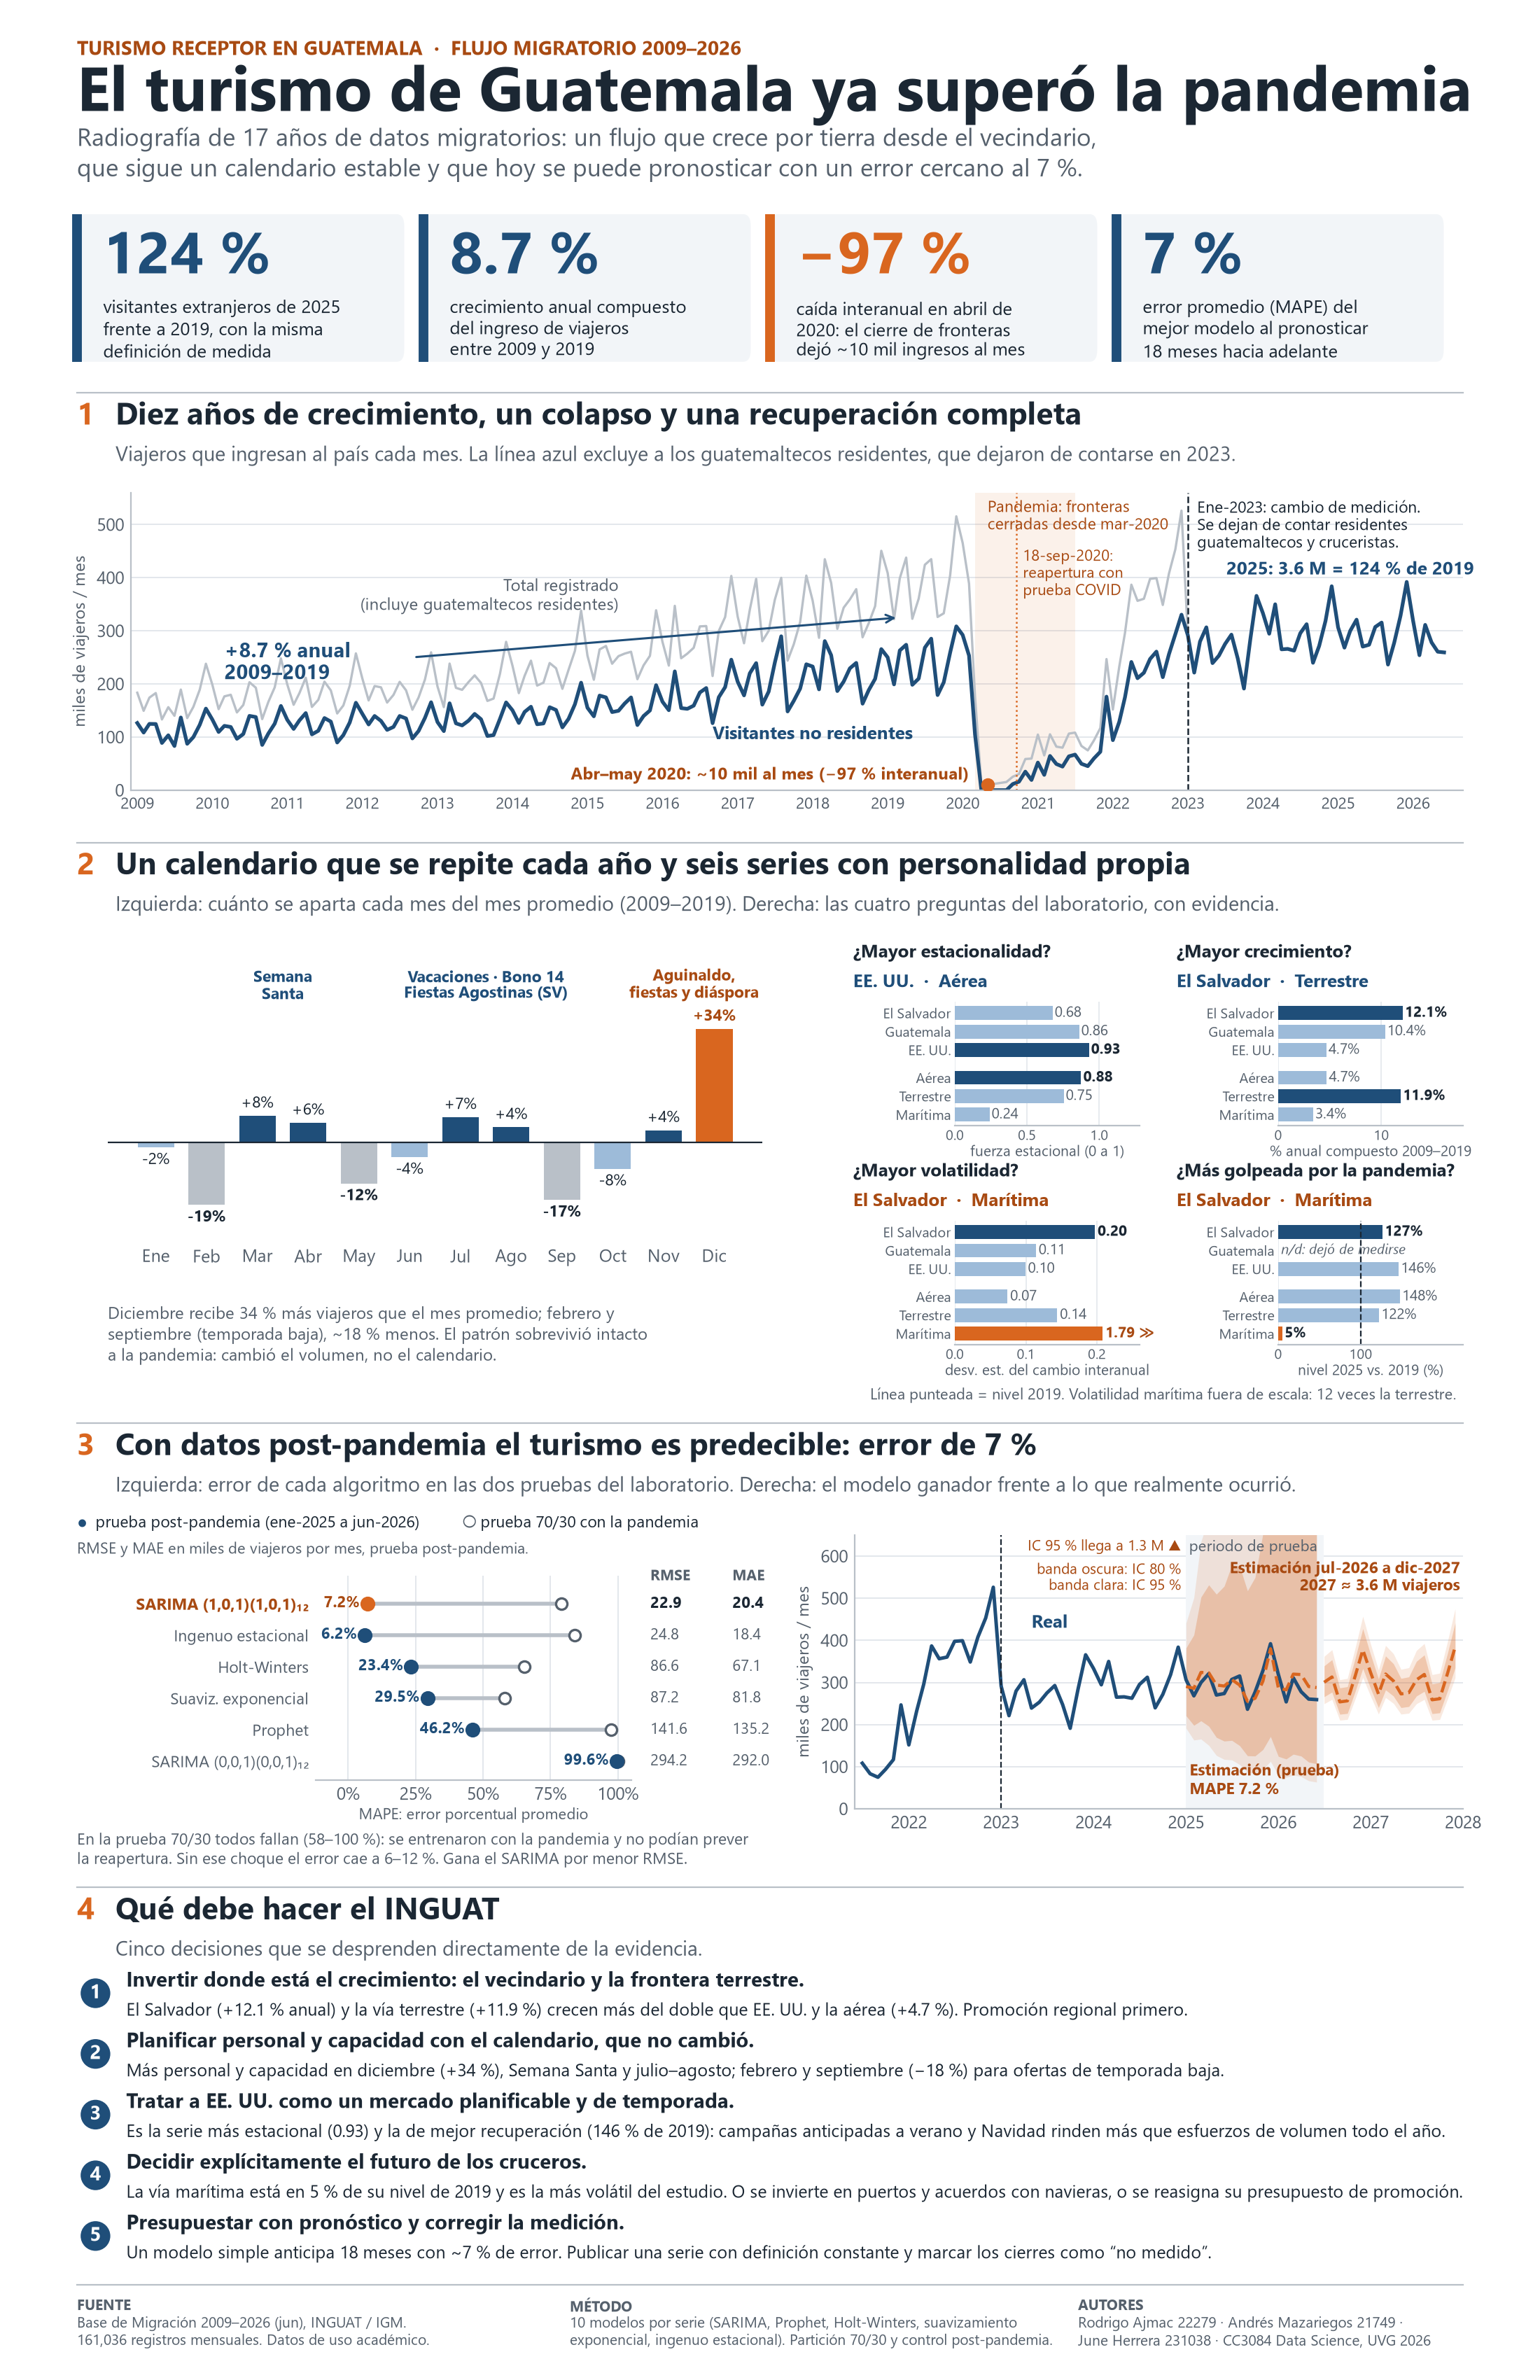
\includegraphics[height=0.86\textheight]{../salidas/infografia.png}
\caption{Versión de avance de la infografía.}
\end{figure}

\end{document}
